\chapter{Desenvolvimento \label{chap:Desenvolvimento}}

% Resumo opcional. Comentar se não usar.
% \resumodocapitulo{Resumo opcional.}


\section{Biblioteca} \label{sec:lib}

O servidor da partida apresenta, como já mencionado, um protocolo de comunicação e sintaxe de mensagens específica. Uma biblioteca de interfaceamento foi desenvolvida com o objetivo de abstrair os detalhes de comunicação de construção de mensagens e facilitar, assim, o desenvolvimento dos programas jogadores. Esta abordagem já é comum na categoria e existem soluções de código aberto como a \textit{librcsc}, utilizada por várias equipes, usualmente atreladas ao agente base \textit{agent2d}, desenvolvidas pela equipe \textit{HELIOS}.

A biblioteca própria foi desenvolvida em linguagem Go como forma de modernização e diversificação da base de código utilizada pelas equipes. A biblioteca cobre uma parte considerável das possibilidades previstas no protocolo de comunicação e foi programada de modo a ser facilmente expansível de acordo com o lançamento de novas versões do servidor.

\subsection{Arquitetura}
A biblioteca possui três pacotes internos: \textit{playerclient}, \textit{trainerclient} e \textit{rcsscommon}. Os dois primeiros dizem respeito aos dois tipos de programas que podem se conectar ao servidor da partida: jogadores e treinadores. O terceiro engloba todas as funcionalidades utilizadas por ambos clientes, além de informações gerais sobre parâmetros da partida, como coordenadas de bandeiras do campo e modos de jogo.

Os dois clientes desenvolvidos possuem as funcionalidades necessárias para se conectar ao servidor, ouvir mensagens via protocolo UDP, decodificá-las e então executar uma ação em forma de mensagem codificada e enviada ao servidor.

\subsection{Decodificação de Codificação de Mensagens}
% lexer -> analisador léxico
% parser -> analisador sintático
A decodificação de mensagens, por sua vez, foi feita em duas camadas: um analisador léxico e um analisador sintático. O lexer passa pelas mensagens em formato string e retira todas as informações que ela contém. O analisador sintático estrutura essas informações em estruturas de dados para que possam ser utilizadas fora da biblioteca. As informações recebidas e decodificadas são, em sua maioria, dados dos sensores do jogador.
\begin{center}



\begin{tabular}{c}
\begin{lstlisting}
(see 37 ((f c b) 16.6 -1 -0 -0.8))
\end{lstlisting}
\end{tabular}

Exemplo de mensagem codificada.


\begin{tabular}{c}
\begin{lstlisting}
SightSymbols{
	Time: 37,
	ObjMap: map[string][]string{
		"f c b":    {"16.6", "-1", "-0", "-0.8"},
	},
}
\end{lstlisting}
\end{tabular}

Mensagem após passar pelo analisador léxico.



\begin{tabular}{c}
\begin{lstlisting}
SightData{
	Time: 37,
	Ball: nil,
	Lines: LineArray{},
	Flags: FlagArray{
		{
			ID:        rcsscommon.FlagCenterBot,
			Distance:  16.6,
			Direction: -1,
		},
	},
}
\end{lstlisting}
\end{tabular}

Mensagem após passar pelo analisador sintático.

\end{center}

\section{Experimentos}

\subsection{Ambiente de Treinamento}

O ambiente de treinamento consiste em uma base de código que importa a biblioteca detalhada na seção \ref{sec:lib}. Um formato geral foi definido e desenvolvido a fim de tornar os experimentos fáceis de adaptar, bastando mudar alguns trechos do código.

Além disso, para os dados disponíveis por meio da biblioteca foram estimados outros estados que pudessem ser úteis no treinamento: posições absolutas da bola, dos outros jogadores e do próprio jogador.

\subsubsection{Laço de Treinamento}

De forma geral o laço de treinamento obedece o pseudo-código apresentado.

\begin{tabular}{c}
	\begin{lstlisting}
definir parametros
inicializar pesos de treinamento
enquanto o estado nao e terminal:
	conectar jogador
	laco para cada passo da partida:
		escolher acao de acordo com a politica e o estado
		observar novo estado e recompensa
		treinar pesos
		estado <- novo estado
	\end{lstlisting}
\end{tabular}

O laço interno é onde efetivamente os algoritmos de treinamento são implementados, portanto este trecho é alterado a depender da técnica de aprendizagem por reforço utilizada.

\subsubsection{Estimação de Estados}

Os sensores do jogador fornecem somente informações em coordenadas polares relativas ao próprio jogador. Desta forma, ele possui informações de distância e direção para a bola, demais jogadores, bandeiras do campo e linhas do campo. 

Com esses dados, entretanto, é possível estimar as coordenadas cartesianas absolutas no campo de todas as entidades de interesse. As bandeiras do campo são fixas e possuem coordenadas conhecidas. Portanto, a transformação da informação polar e relativa para uma cartesiana e absoluta da posição do próprio jogador é direta utilizando trigonometria básica. 

A partir da informação de posição absoluta do próprio jogador e de sua direção é possível calcular as posições para o resto das entidades.

\subsection{Agente Único com Double Q-Learning Tabular}

% Inicialmente, deseja-se realizar o treinamento de um agente único que, com as informações de seus sensores, consiga com sucesso levar a bola ao gol. Essa proposta tem como objetivo fundamentar os conhecimentos e validar a base de código para a realização de um treinamento de um time de múltiplos agentes em um estágio posterior.

% O desenvolvimento de um agente único, inicialmente, permite adquirir o entendimento necessário para a definição do vetor de estados e ajuste das técnicas de treinamento. Além disso, busca-se uma maior agilidade na substituição e teste na estrutura do vetor de estados e no algoritmo de treinamento, uma vez que o custo computacional deste cenário é consideravelmente menor que o custo do treinamento de um time completo.

O objetivo inicial para teste do sistema como um todo foi o de realizar o treinamento de um agente único capaz de executar gols estando sozinho em campo. Esse objetivo se provou mais difícil do que o esperado para a abordagem \textit{end-to-end} desejada.

Foi utilizado o algoritmo Double Q-Learning tabular, possível através da discretização de diversas métricas obtidas através dos sensores do agente.

\subsubsection{Codificação dos Estados}

O estado percebido pelo agente é dado pela combinação dos seguintes fatores:

\begin{itemize}
    \item \textbf{Distância até a bola}. A distância $D$ até a bola foi discretizada de acordo com a seguinte função:
    \begin{equation}
    \label{eq:balldist}
    \left\{
        \begin{array}{ll}
            0  & \mbox{se } D < 0.7 \\
            \lfloor\log_2 (\frac{D}{0.7})\rfloor & \mbox{se } 0.7 \leq D \mbox{ e } D < 0.7 \times 2^6 \\
            6  & \mbox{se } D \geq 0.7 \times 2^6 \\

        \end{array}
    \right.
    \end{equation}

    Ou seja, a distância percebida até a bola varia entre 0 e 6 com resolução cada vez menor à medida que o agente se afasta da bola. O fator 0.7 foi inserido na função devido ao fato de que esta é a distância mínima que permite que o agente chute a bola.

    Caso o jogador possa enxergar a bola, a distância D é recebida diretamente do sensor. Caso contrário, a distância D é estimada com base na última posição percebida da bola.

    \item \textbf{Direção da bola}: A direção da bola foi dividida em 24 fatias de $15^{\circ}$ cada. O ângulo de visão do jogador é de $\pm30^{\circ}$. Caso a bola não esteja visível, a direção da bola é estimada com base na última posição percebida.
    
    \item \textbf{Posição do jogador em X}: A posição estimada do jogador em X foi discretizada em 10 janelas de tamanho $11.5$.

    \item \textbf{Posição do jogador em Y}: A posição estimada do jogador em Y foi discretizada em 7 janelas de tamanho aproximado $11.14$.
    
    \item \textbf{Direção do jogador}: A direção estimada do jogador em relação ao eixo horizontal foi discretizada em 24 fatias de $15^{\circ}$ cada.

\end{itemize}

Com isso, temos que o número total de estados possíveis é dado pelo produtório da quantidade de possibilidades em cada um dos itens acima totalizando 282240 estados.

\subsubsection{Codificação das Ações}

Para simplificar o vasto espaço de ações disponíveis, foi selecionado um conjunto discreto de 13 ações:

\begin{itemize}
    \item \textbf{Ação nula}: O agente apenas espera até o próximo ciclo.

    \item \textbf{Virar-se}: O agente tem a opção de virar-se $7^{\circ}$, $15^{\circ}$ ou $31^{\circ}$ para ambas as direções, totalizando 6 ações de rotação possíveis. 
    
    \item \textbf{Correr}: É possível correr em frente ($0^{\circ}$) ou a $30^{\circ}$ em ambas as direções, sempre com potência 50, totalizando 3 ações de corrida possíveis.

    \item \textbf{Chutar}: Caso a distância até a bola seja menor ou igual a 0.7 metros, o jogador tem a opção de chutá-la em frente ou em um ângulo de $45^{\circ}$ em ambas as direções, totalizando 3 ações de chute possíveis. Caso a bola não esteja próxima o suficiente, nada acontece.
\end{itemize}

\subsubsection{Parâmetros}

\begin{itemize}
    \item \textbf{Fator de desconto ($\gamma$)}: Apesar do ambiente ser episódico, foi utilizado um fator de desconto de 0.99 devido ao fato de que a condição de término do episódio (fim de jogo) não ser observável através da discretização do estado utilizada.  

    \item \textbf{Fator de aprendizagem ($\alpha$)}: O fator de aprendizagem foi definido inicialmente como 0.1 e foi reduzido exponencialmente multiplicando-o por $0.99999$ ao final de cada partida. 
    
    \item \textbf{Fator de exploração ($\epsilon$)}: Para incentivar a exploração das possibilidades, o fator de exploração foi definido inicialmente como 0.9 e reduzido exponencialmente multiplicando-o por $0.99996$ ao final de cada partida. A cada ação tomada, o agente tem probabilidade $\epsilon$ de escolher uma ação aleatória. Além disso, para favorecer a exploração, no início de cada partida era também sorteada uma posição inicial para o agente em seu lado do campo.
\end{itemize}

\subsubsection{Recompensa}

A recompensa foi definida em 3 partes a fim de guiar o agente na direção do aprendizado desejado. Todas as medições de recompensa foram feitas utilizando dados da simulação e não da percepção do agente.

\begin{itemize}
    \item \textbf{Proximidade da bola $R_1$}: Para que o agente tenha tendência a se aproximar da bola, foi definida uma recompensa negativa proporcional à distância $d$ do agente em relação à bola, ou seja: $R_1 = -d*0.001/6000$.

    \item \textbf{Velocidade da bola $R_2$}: Para que o agente adquira o comportamento de chutar a bola em direção ao gol adversário, foi definida uma recompensa positiva proporcional à velocidade instantânea da bola em X ($v_x$), ou seja: $R_2 = v_x/6000$.
    
    \item \textbf{Gol $R_3$}: Por fim, para incentivar que o agente fizesse gols, foi definida uma recompensa esparsa de valor 1 para cada gol realizado e -1 para gols contra, ou seja:
    
    $
    R_3 =
    \left\{
        \begin{array}{ll}
        \ \ 1  & \mbox{se foi feito um gol no ciclo} \\
         -1  & \mbox{se foi feito um gol contra no ciclo} \\
        \ \ 0  & \mbox{caso não houver gol no ciclo} \\
        \end{array}
    \right.
    $
\end{itemize}

Deste modo, a cada instante de tempo foi atribuída uma recompensa $R = R_1 + R_2 + R_3$.

\subsubsection{Procedimentos e Resultados}

Foram executados 2 treinamentos distintos de 100000 partidas a fim de suavizar o elemento sorte nos resultados. Após cada um dos treinamentos foi salva a tabela Q completa e o histórico dos retornos obtidos pelo agente ao longo do treinamento.

Os gráficos a seguir mostram esse histórico. É interessante observar que com o decaimento dos fatores de exploração e de aprendizagem, após 100000 partidas ambos eram $\epsilon \approx 0.01648$ e $\alpha \approx 0.03679$, ou seja, o agente já executava na maior parte dos ciclos a política ótima aprendida.

\begin{figure}[h]
	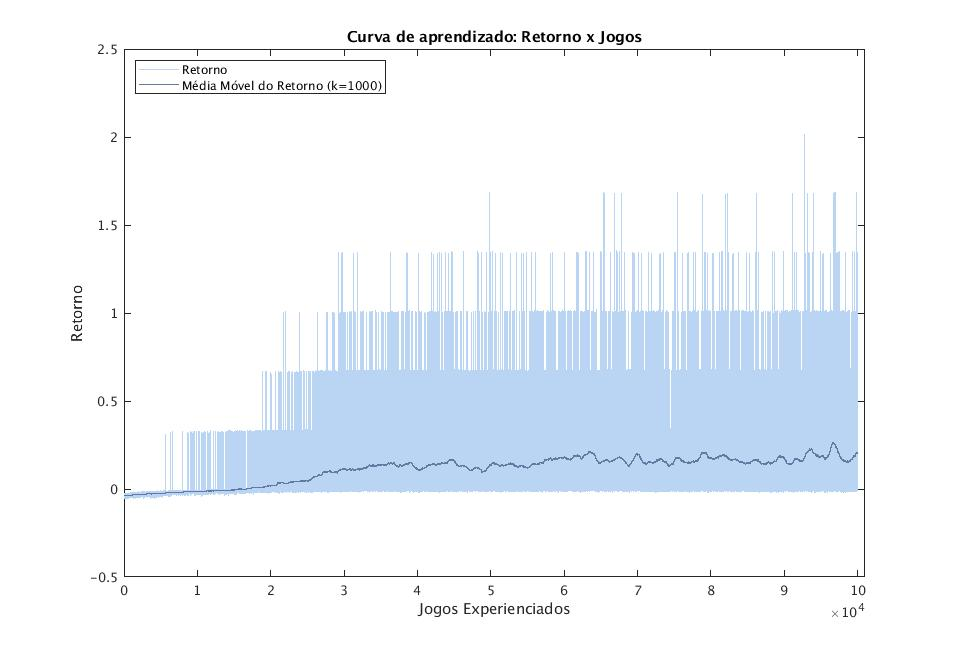
\includegraphics[width=1.0\linewidth]{figs/curva-qtabular.jpg}
	\centering
	\caption{Curva de aprendizado. Para cada jogo foi feita a média entre os 2 retornos observados em cada um dos treinamentos.}
	\label{fig:single-agent-curva}
\end{figure}

% \section{Agentes Concorrentes}

% Após validação do sistema com agente único, é interessante experimentar com treinamento adversarial de apenas 2 jogadores em formato um-contra-um. A intenção dessa etapa é experimentar com o sistema o caso adversarial, no qual há um ou mais agentes com objetivo oposto ao do agente sendo treinado.

% \section{Múltiplos Agentes}

% Após validar os casos de agente único e de agentes concorrentes, propõe-se um treinamento completo em jogos 11 contra 11. O objetivo é, ao final do processo, termos um time capaz de jogar contra os principais times da atualidade na categoria RoboCup Soccer Simulation 2D.

% Para isso, os agentes devem ser capazes de cooperar e reagir aos movimentos da equipe oposta a fim de marcar gols e evitar os gols do adversário.
